% Mode d'emploi: Switcher les deux lignes suivantes pour passer du
% mode présentation au handout
% ===================================================
\documentclass[ignorenonframetext,red]{beamer}
%\documentclass[12pt]{article} \usepackage{beamerarticle} \usepackage{fullpage}
% ===================================================

\usepackage{ucs}
\usepackage{mathpartir}
\usepackage{amsfonts,amsmath,amscd}
\usepackage{stmaryrd}
\usepackage[utf8x]{inputenc}
\usepackage[protrusion=true,expansion=true]{microtype}
\usepackage{setspace}
\usepackage{graphicx}

\title{Towards typed repositories of proofs \\[0.6em] 
  \small \textsf{MIPS 2010}}

\date{July 10, 2010}

\author[Matthias Puech \& Yann Régis-Gianas] {
Matthias Puech\inst{1} \and Yann Régis-Gianas\inst{2} \\
{\small \url{puech@cs.unibo.it}} \and {\small \url{yrg@pps.jussieu.fr}}
}
\institute {
  \inst 1 {\small Dept. of Computer Science, University of Bologna} \and
  \inst 2 {\small University Paris 7, CNRS, and INRIA, PPS, team ${\pi}r^2$}
}

\setbeamertemplate{footline}[frame number]
\setbeamertemplate{navigation symbols}{}

% \AtBeginSection[]
% {\begin{frame}<beamer>{Outline}
%     \tableofcontents[currentsection]
%   \end{frame}
% }

\usefonttheme{serif}

\begin{document}

\begin{frame}
  \titlepage
  \mode<article>{
    \newcommand\url\texttt
    \maketitle}
\end{frame}

\section{Motivation}

I am going to present a work-in-progress, realized together with Yann
Régis-Gianas. It is far from a finished product, so feel free to
interrupt, comment or criticize. So this talk will be about some
observations and directions to improve the way we edit and store
formal proofs in proof assistants.

\hrule
\begin{frame}{How are \emph{constructed} formal mathematics?}
  \large
  \begin{tabular}{ll}
    {\Huge Q :} & \parbox{0.8\textwidth}{What is the common point between the working
      mathematician and the working programmer?} \\[2em]
    \pause
    {\Huge A :} & They both spend more time \emph{editing} than \emph{writing}
  \end{tabular}
\end{frame}
\hrule

Let me start with a simple observation relating the activity of both
the working mathematician and the computer scientist. Both activities
could be percieved, from the outside, as apodictic because the final
object of their study, the proof or the program, seems to be
unquestionably valid (or not).

If we observe the day-to-day work of these scientists though, their
workflow resembles a lot more that of experimental sciences: it is
highly non-linear, involving multiple parallel experiments, fixes,
backtrack on previous modifications\ldots\ eventually validated or
invalidated by some \emph{a posteriori} criterion, the absence of
bugs, the validity of a proof.

In other words, the mathematician and the programmer spend more time
\emph{editing} their developments non-linearly than monotonously
\emph{writing} new material.

It is the case for programs, for classical, paper mathematics so it
should be the case for formal mathematics, edited in a proof
assistant.

\hrule
\begin{frame}{A paradoxical situation}  
  \begin{block}{Observation}
    Workflow of formal mathematics was largely inspired by software
    development:
    \begin{itemize}
    \item File-based scripts (\textsf{emacs})
    \item Separate compilation (\textsf{make})
    \item Text-based versioning (\textsf{svn}, \textsf{diff}s\ldots)
    \end{itemize}
  \end{block}
  \pause
  \begin{block}{\ldots\ And yet,}
    Powerful tools to mechanize the metatheory of (proof) languages
  \end{block}
  \vspace{0.6em}
  \pause
  \begin{center}
    {\large \it Isn't it time to make these tools metatheory-aware?}
  \end{center}
\end{frame}
\hrule

Since the advent of modern proof assistants, large bodies of
mathematics have been formalized and the way people managed these
developments is very similar to the one used in software development
for years: we write proofs in text files, which are linear, and launch
proof-checking when we are done. To avoid re-checking the whole
development, we split it into inter-dependent files and re-check only
those who have changed. To keep track of old versions, we use
line-based version control systems that have no awareness of the
actual content of the files. In a sense, the non-linearity of proof
development is managed outside the scope of the tool, by manual,
textual transformations that are often very unsatisfactory.

The paradox about this situation is that these very tools (Coq,
Matita, Agda) can be used to reason about formal languages and
especially proof languages, some of these tools are even dedicated to
the mechanization of the metatheory of proof languages. But we still
use this legacy generic tools to manage our developments.

Couldn't we adapt the methods developed to reason about formal
languages to the language of the proof assistant itself? Could we
replace this legacy toolchain and make it language-aware, even
semantic-aware?

\hrule
\begin{frame}{Motivations}
  \begin{block}{Rigidity of linear edition}
    \begin{itemize}
    \item ((edit; compile)*; commit)* loop does not scale to proofs
    \item Concept freeze inhibits the discovery process
    \item No room for alternate definitions
    \end{itemize}
  \end{block}
  \pause
  \begin{block}{Laxity of textual representation}
    \begin{itemize}
    \item Textual scripts \textsf{diff}s do not reflect the semantics
    \item Not even the syntax
    \end{itemize}
  \end{block}
  \vspace{2em}
  \pause
  {\tiny \ldots\ Maybe it wasn't adapted to software development}
\end{frame}
\hrule

More precisely, here are some problems that arise with the traditional
tools when editing proofs. Whereas the usual edit, compile, commit
loop may be a satisfactory approximation when developing software, the
extra computational cost of proof-checking makes it unsatisfactory as
the development grows: often the time of recompilation is prohibitive.

But it is not only a matter of time: once a concept is proof-checked,
it is frozen and any future modification of it will require to
re-check a large part of the development, often much more than what is
actually required. We believe that this fact inhibits the use of proof
assistants as tools to help the mathematician in the discovery
process, as an experimentation tool, and not only to formally
transcribe paper proofs.

The same way, the linearity of proof scripts does not allow any
flexibility in the alternate definition of concepts.

On the other side, the way we store mathematical developments, that is
as textual files or textual diffs does not reflect neither their
syntax nor their semantics, and as I will try to show, there is a lot
to gain in changing this base representation.

In fact, some will say that this model of interaction wasn't even
adapted to programming in the first place.

\hrule
\begin{frame}{The impact of changes}
  \vspace{0.5em}
  \begin{center}
    \only<1>{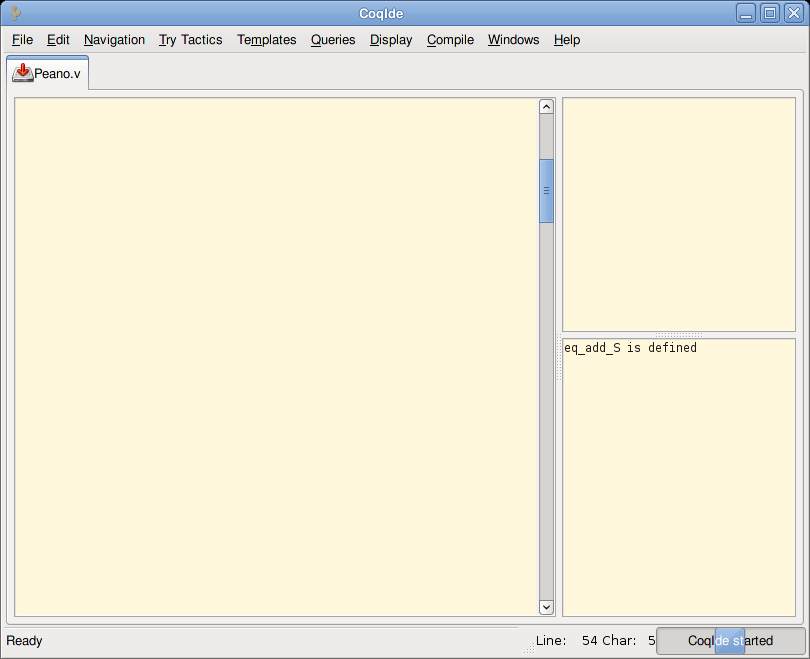
\includegraphics[width=0.75\textwidth]{images/coqide00.png}}%
    \only<2>{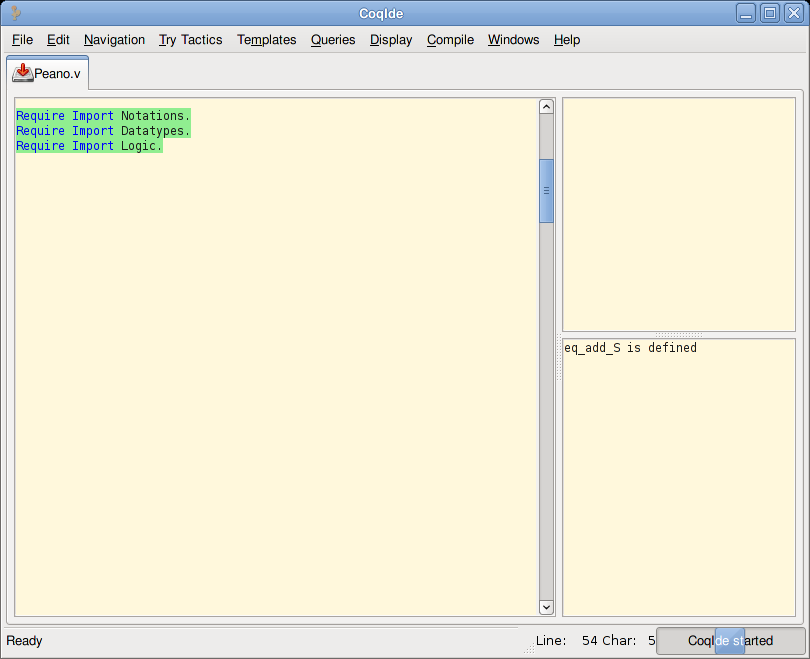
\includegraphics[width=0.75\textwidth]{images/coqide0.png}}%
    \only<3>{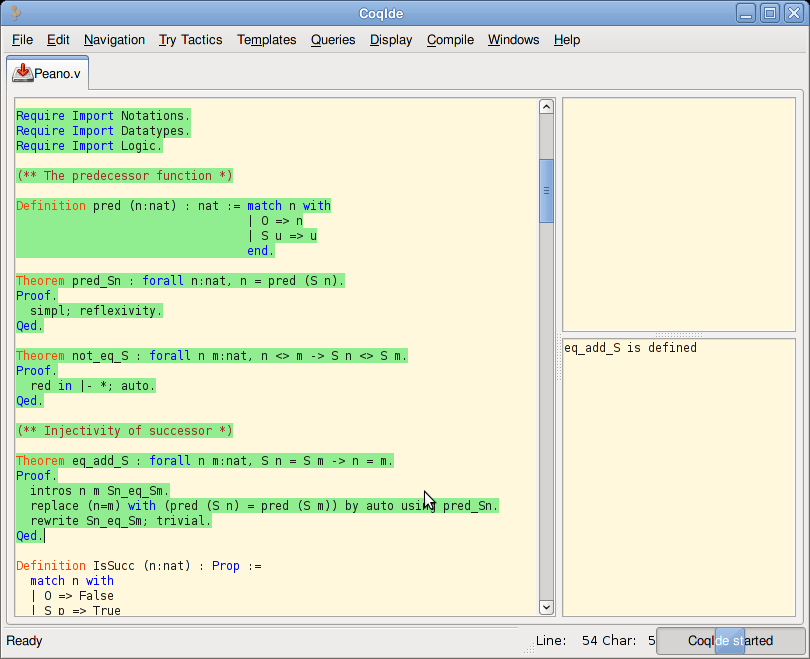
\includegraphics[width=0.75\textwidth]{images/coqide.png}}%
    \only<4>{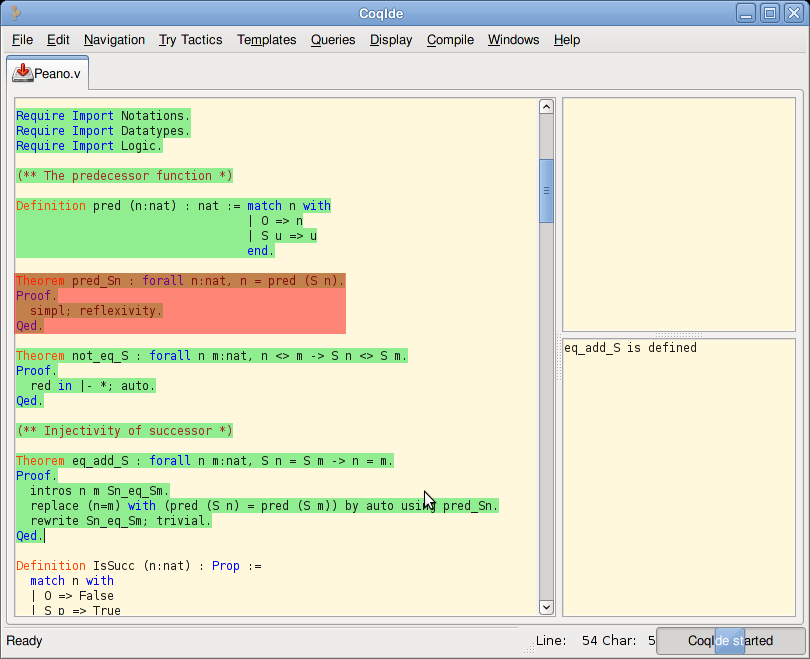
\includegraphics[width=0.75\textwidth]{images/coqide2.png}}%
    \only<5>{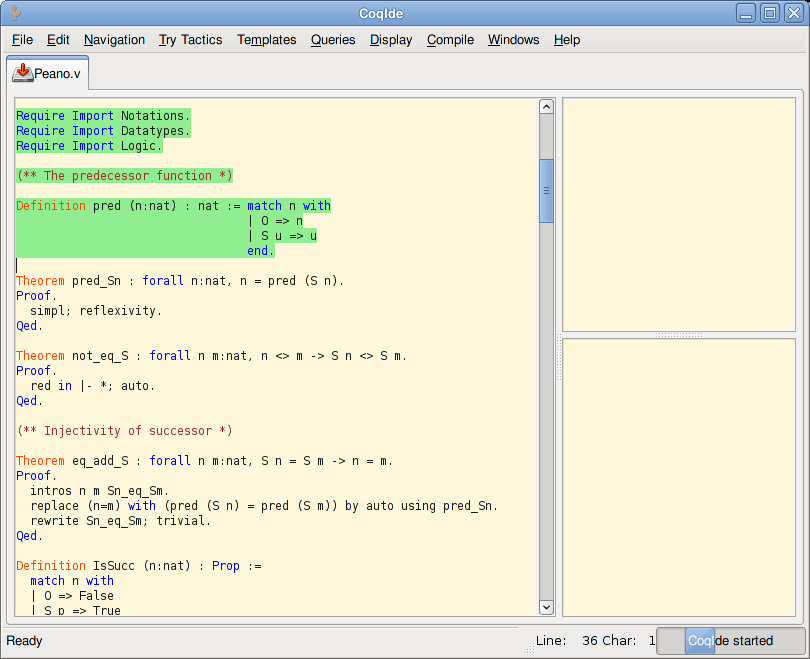
\includegraphics[width=0.75\textwidth]{images/coqide4.png}}%
    \only<6>{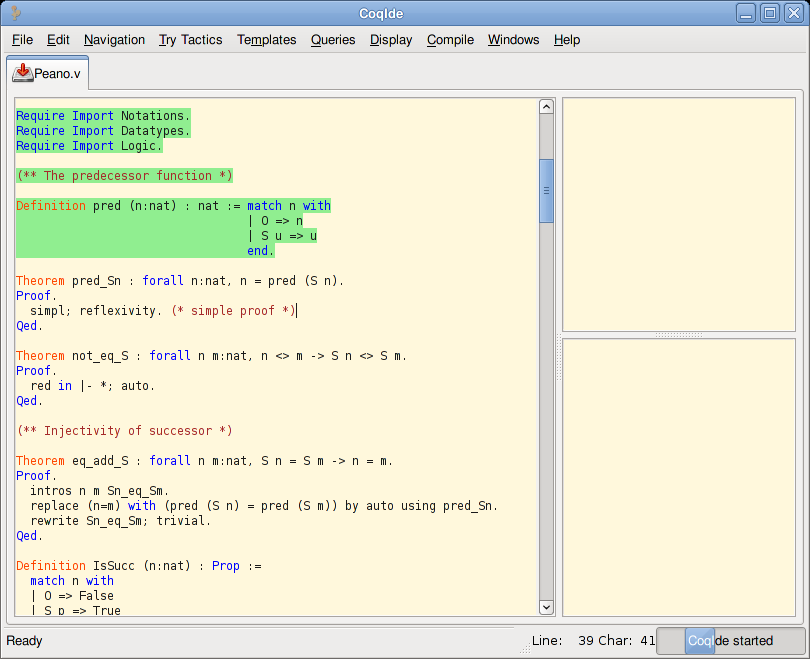
\includegraphics[width=0.75\textwidth]{images/coqide5.png}}%
    \only<7>{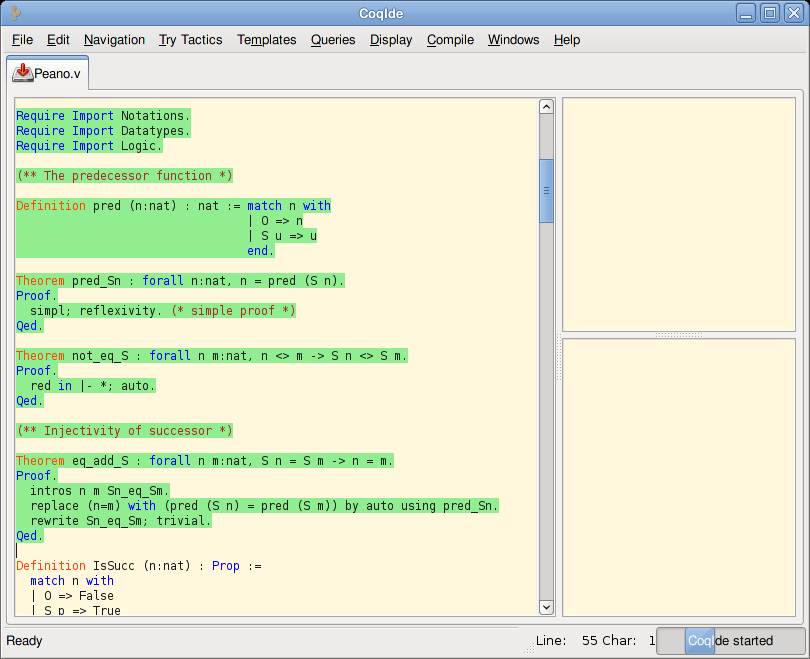
\includegraphics[width=0.75\textwidth]{images/coqide6.png}}%
    \only<8>{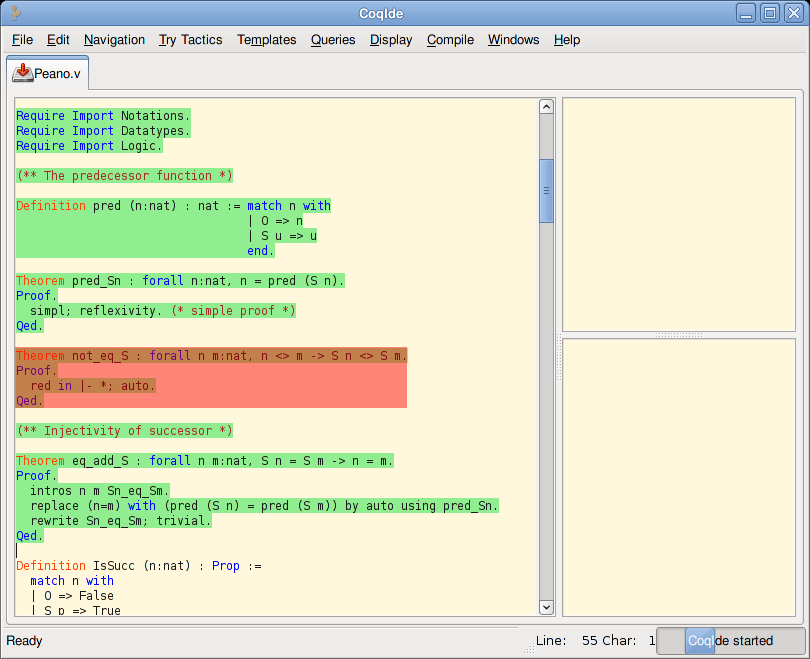
\includegraphics[width=0.75\textwidth]{images/coqide7.png}}%
  \end{center}
  \pause
  \uncover<2->{
    \begin{itemize}
    \item File-based separate compilation
      \pause
    \item Interaction loop with global undo
    \end{itemize}
  }
\end{frame}
\hrule

We can then see a number of extra-logical features of modern proof
assistants as ways to cope with these problems. 

Instead of writing our complete development in one unique file and let
the program check it when done, we can split it in several files or
modules and establish dependencies among them: only those who changed
(and their dependencies) have to be rechecked.

But this separation serves two different purpose, and the fact that
they coincide is pure contingency: the purpose of splitting a
development into logical units, and the purpose of providing a coarse
notion of dependency to ease the non-linear process of proof editing
by accelerating recompilation upon changes.

Secondly, the traditional interaction loop makes unnecessary the
recompilation upon local changes by providing a global undo feature of
the whole state of the proof assistant. But if I want to change this
proof, I have to backtrack all the way here (because the green region
is locked), do my changes and then replay the whole proofs in between,
even if my change had no impact on this one, even if I just added a
comment.

The actual text of the proofs for versioning is often
non-satisfactory: on one side it contains mostly non-relevant
informations (line breaks, spaces\ldots), on the other the relevant
ones, the validity of the proof, the dependency between objects, is
absent.

So both these facilities, among others, seem to provide ad-hoc ways to
deal with the non-linearity of the script and its edition. They
provide a coarse approximation of the dependency amongst objects. But
this notion of dependency \emph{is} a metatheoretical property of a
logic, and it could be used to provide an \emph{exact} way of dealing
with the impact of changes, in particular to guide proof-checking to
recheck only minimal parts of the developments.

This is what we will try to do in the following.

\hrule
\begin{frame}{Methodology}
  \begin{center}
    \only<1-2>{\fbox{\parbox{20em}{\only<2>\alert{version
            management}\\[1em]%
          \fbox{\parbox{18em}{script files\\[1em]%
              \fbox{\parbox{17em}{parsing\\[1em]%
                  \fbox{\parbox{14em}{proof-checking\\} }}}}}}}}%
    \only<3>{\fbox{\parbox{20em}{script files\\[1em]%
          \fbox{\parbox{18em}{\alert{version management}\\[1em]%
              \fbox{\parbox{17em}{parsing\\[1em]%
                  \fbox{\parbox{14em}{proof-checking\\} }}}}}}}}%
    \only<4->{\fbox{\parbox{20em}{\alt<-5>{script files}{user
            interaction}\\[1em]%
          \fbox{\parbox{18em}{parsing\\[1em]%
              \fbox{\parbox{17em}{\alert{version management
                    \only<7->{+ proof-checking}}\\[1em]%
                  \uncover<4-6>{\fbox{\parbox{14.5em}{proof-checking\\}}}}}}}}}}%
  \end{center}
  \begin{itemize}
  \item<4-> AST representation
  \item<5-> Explicit dependency DAG
  \item<7-> Typing annotations
  \item<8-> Incremental type-checking
  \end{itemize}
\end{frame}
\hrule

Here is a schematic view of the traditional way to manage formal
developments. The user writes scripts which are version controlled,
and these scripts are parsed and checked on demand. By pushing version
management inwards, we abstract from syntax, and more informations
become available. For instance we can compute the acyclic graph of
dependencies. At this level already, the situation is greatly
enhanced: syntax, and file-based development, get the place they
deserve: they are relegated to a tool for user interaction, the actual
development being stored and manipulated in an abstract form. We could
even imagine syntax being dynamically switchable, part of user
preferences!

But let's go one step further and embed version management into the
type-checker. We gain access to type informations at the level of
changes, that is, we can track changes, dependencies and types at the
same time, and decide to type-check only local changes of the
development and their global effect, in a minimal way. We can perform
\emph{incremental type-checking}.

\hrule
\begin{frame}{A core meta-language for incremental type-checking}
  \begin{columns}[t]
    \begin{column}{0.5\textwidth}
      \begin{block}{Expresses}
        \begin{itemize}
        \item (abstract) Syntax
        \item (object-) Logics
        \item Proofs (-terms)
        \end{itemize}
      \end{block}
    \end{column}
    \begin{column}{0.5\textwidth}
      \begin{block}{Features}
        \begin{itemize}
        \item Typing
        \item Incrementality
        \item Dependency
        \end{itemize}
      \end{block}
    \end{column}
  \end{columns}
  \vspace{2em}
  \begin{center}
    \emph{A kernel for a typed version control system?}
  \end{center}
\end{frame}
\hrule

In the following, I will present a preliminary implementation of these
ideas. It is a meta-language for incremental proof-checking, that is a
language in which one can define abstract syntaxes, logical rules and
proofs, and allows to check validity, express the incrementality of
the constructions, and their dependency. It can be viewed as a kernel
for a generic, typed version control system, and for the first
iteration of this project, we were inspired by the way \textsf{git}
stores the history of directories.

\hrule
\begin{frame}{Inspiration: the \textsf{git} storage model}
  \begin{center}
    \begin{overlayarea}{\textwidth}{12em}
      \only<2>{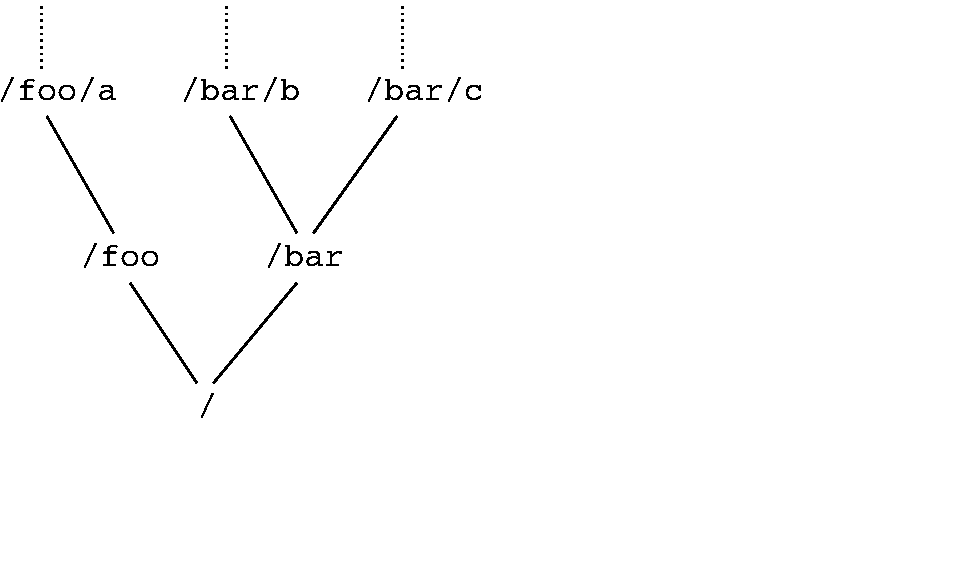
\includegraphics[width=0.85\textwidth]{images/git1.pdf}}%
      \only<3>{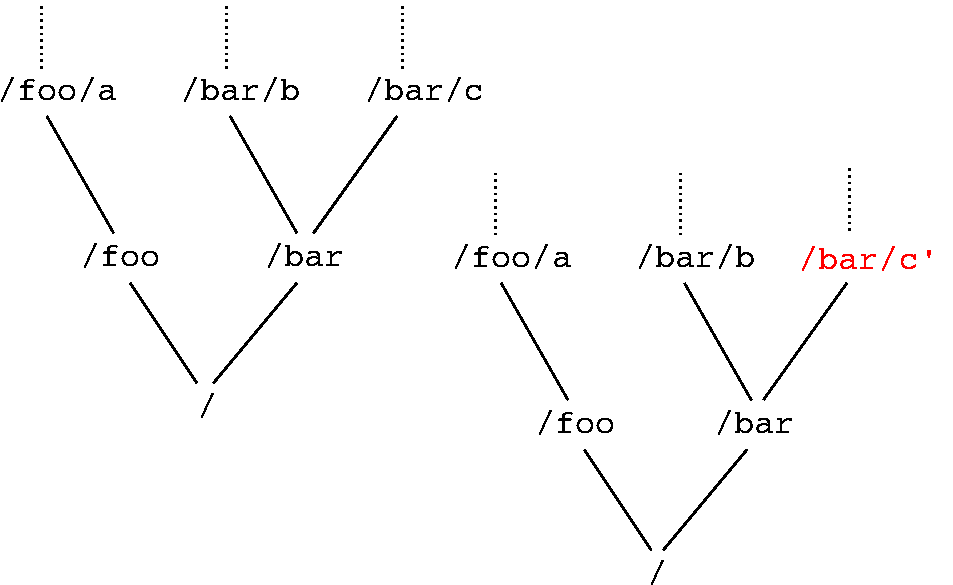
\includegraphics[width=0.85\textwidth]{images/git2.pdf}}%
      \only<4>{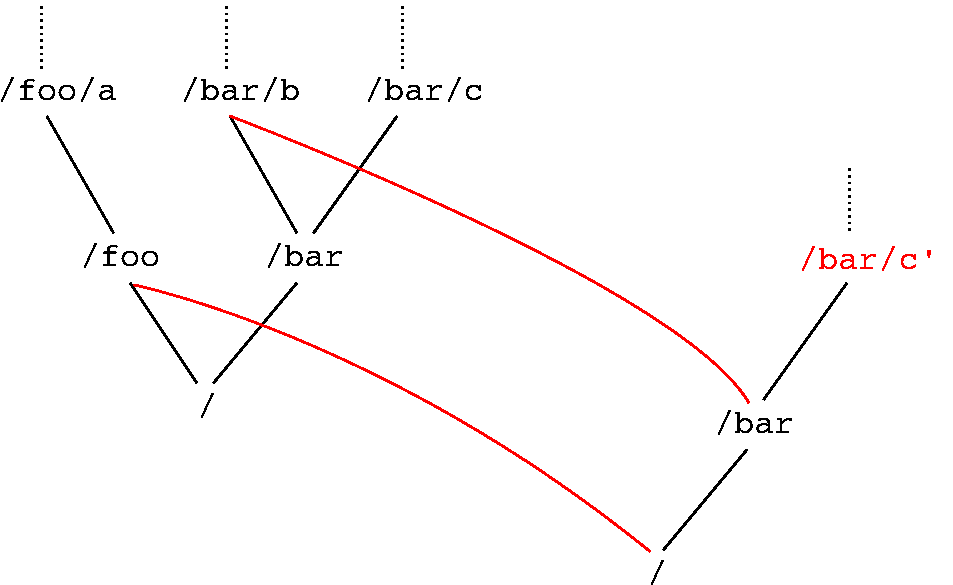
\includegraphics[width=0.85\textwidth]{images/git3.pdf}}%
      \only<5>{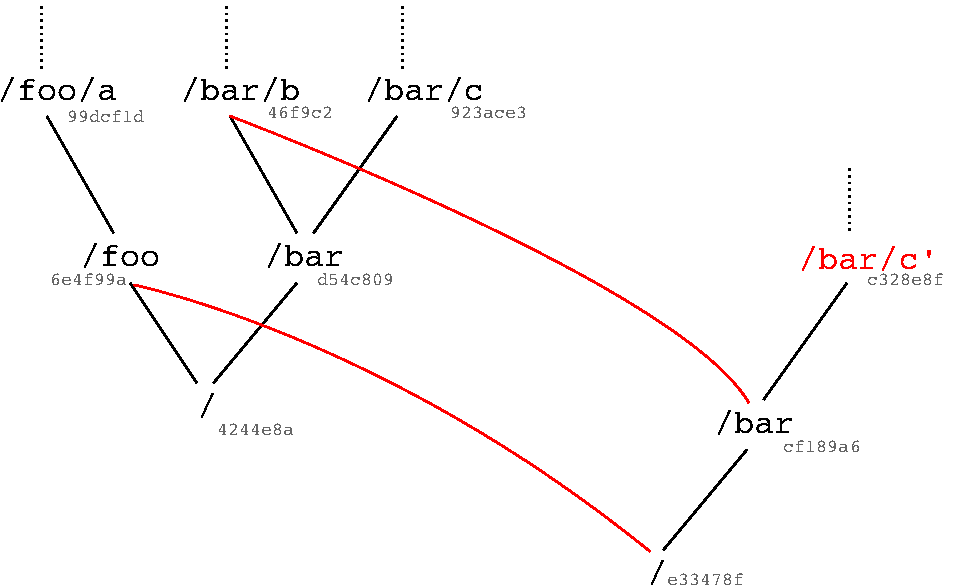
\includegraphics[width=0.85\textwidth]{images/git4.pdf}}%
      \only<6-9>{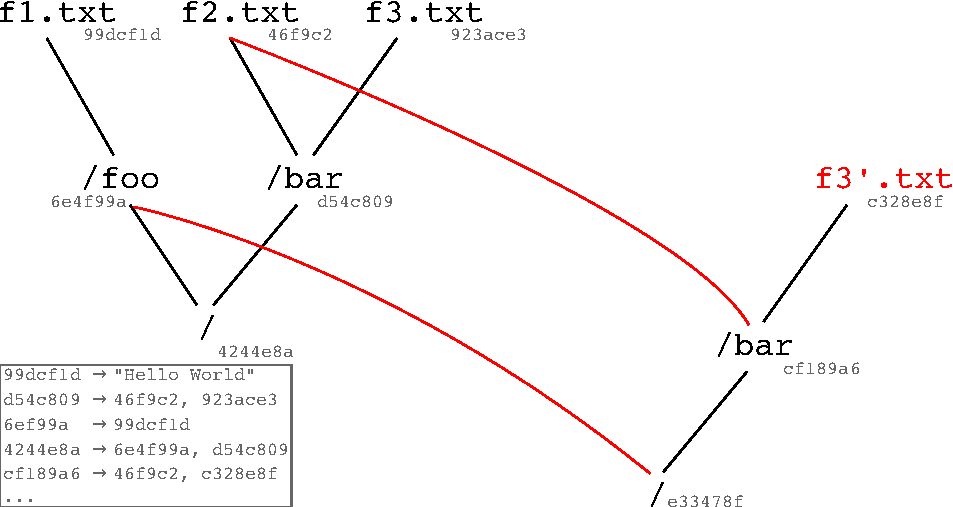
\includegraphics[width=0.85\textwidth]{images/git5.pdf}}%
      \only<10>{
        \begin{center}
          \vspace{5em}
          {\Large Let's design a \emph{typed} \textsf{git}}
        \end{center}
      }%
    \end{overlayarea}
  \end{center}%
  \begin{itemize}\small %
  \item<7-> ``Content-adressable''%
  \item<8-> Name reflects content%
  \item<9-> Maximal sharing (or hash-consing)%
  \end{itemize}%
\end{frame}
\hrule

\textsf{Git} is one of the most successful version control system, and
part of its success is due to the very simple, yet very powerful
storage model. It doesn't keep track of changes \emph{per se}, but of
similarities between version. Given a base directory structure,
already committed in its database, and a new version of it with, let's
say, one file changed -- \texttt{f3.txt}, it stores the new version by
linking all common subdirectory structure to the previous
version. This way, similarities are physically relalized by this kind
of ``compression''. This is possible because every node in the tree,
directories and files, have a unique name. So actually, the database
of \textsf{git} looks like this: it associates to every name, a
content (for files) or a list of names (for directories). The
invariant is that this database forms a DAG. This naming policy makes
all content adressable.

Moreover, similarities are easily tracked because every name is
carefully chosen to reflect the \emph{content} of a file or directory.
In practice, \textsf{git} uses a hash function to produce all names in
the database: files are given the hash of their content, and
directories are given the hash of the hash of all the files it
contains, recursively.

This way, we ensure that no two subdirectories with different content
appear in the database, that is, we enforce maximal sharing among
subdirectories. In functional programming, this is called
hash-consing.

Let's apply the same discipline to proofs, and validate them by
typing. What would we get?

\hrule
\begin{frame}{A typed repository}
  \only<1>{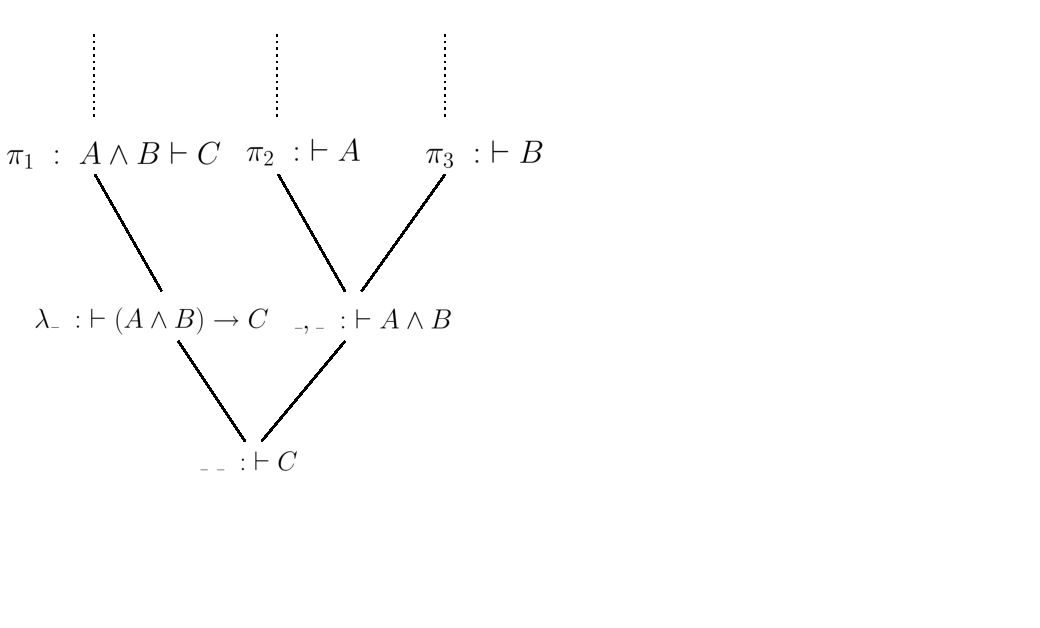
\includegraphics[width=\textwidth]{images/gasp1.pdf}}%
  \only<2>{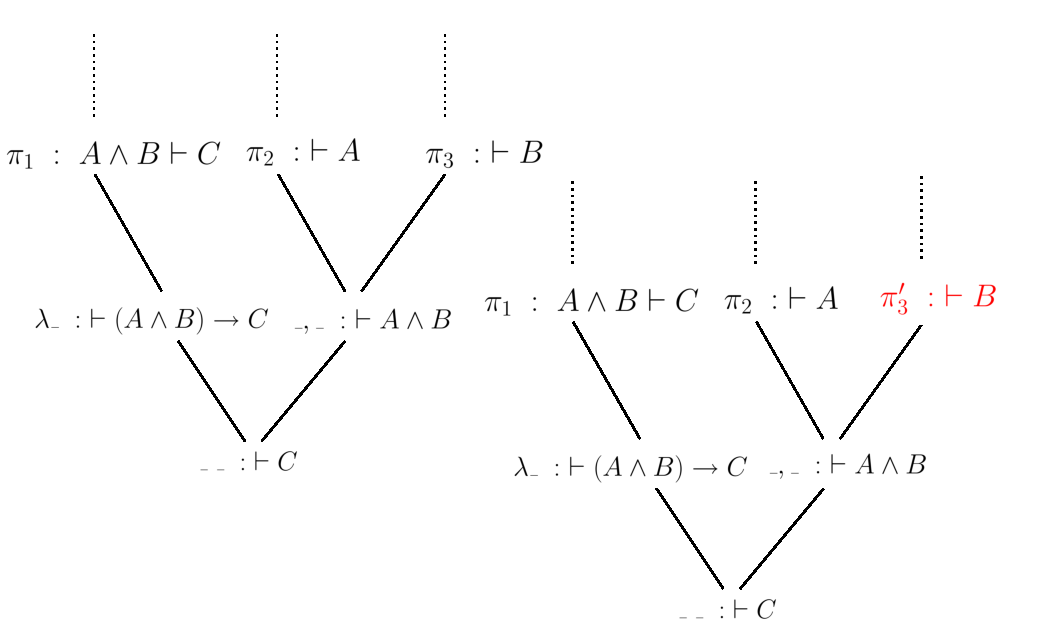
\includegraphics[width=\textwidth]{images/gasp2.pdf}}%
  \only<3>{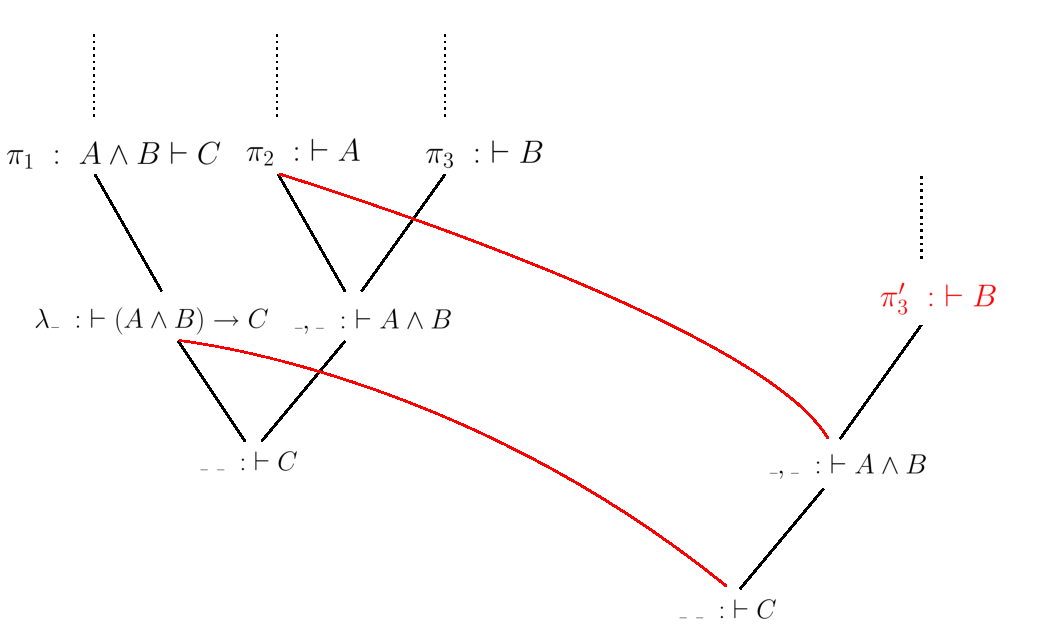
\includegraphics[width=\textwidth]{images/gasp3.pdf}}%
  \only<4>{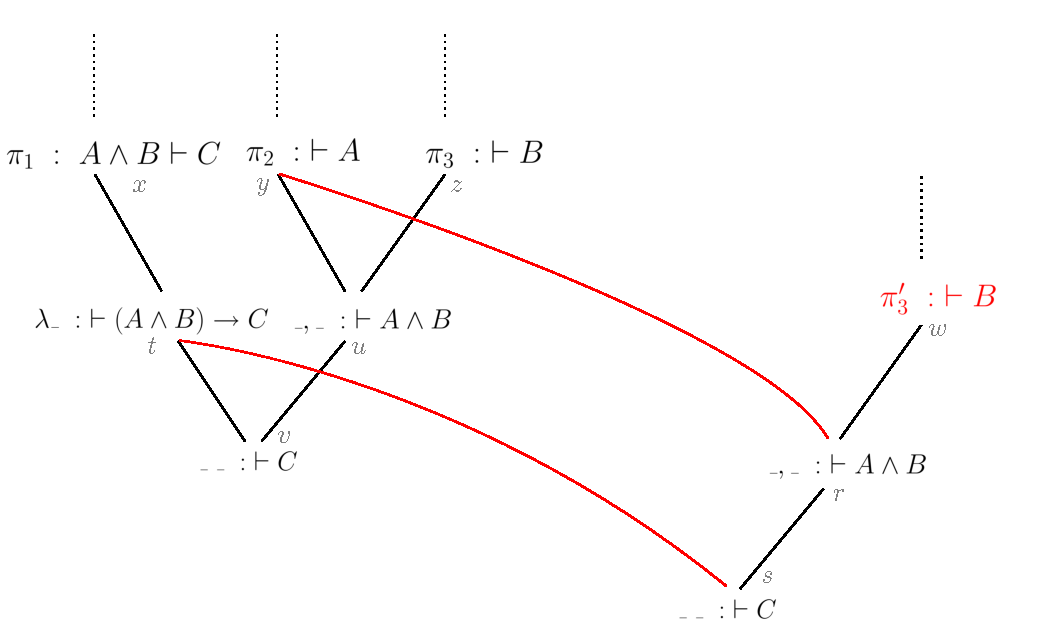
\includegraphics[width=\textwidth]{images/gasp4.pdf}}%
  \only<5>{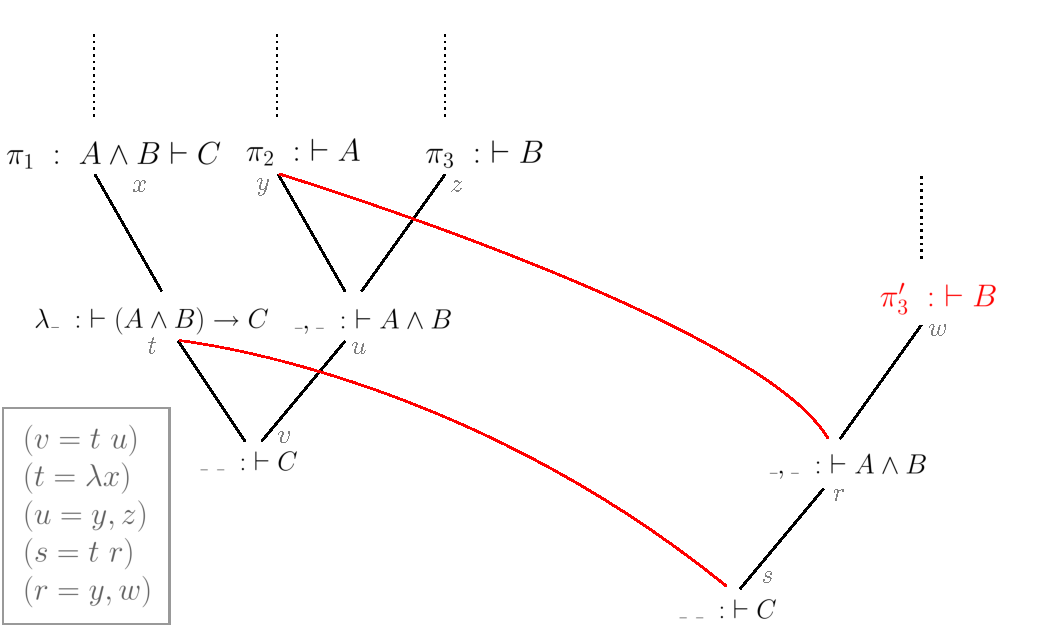
\includegraphics[width=\textwidth]{images/gasp5.pdf}}%
\end{frame}
\hrule

On the same model, let's start with a proof of $C$ already committed,
and starting with this structure. $\pi_1$, $\pi_2$ and $\pi_3$ are the
rest of the proof, upwards. Each node is labelled with the logical
rule (or constructor) used, but also annotated by the judgement it
proves. Now let's imagine that we come up with a new, better proof for
$B$. Integrating it in the repository means, like before, to share all
common sub-derivations. But now, we don't need to retype the whole new
proof, just the new parts (in red). Like before, this is possible if
we give a name to all sub-derivations, and the database looks like
this: it associates with every name, how it is formed.

\hrule
\begin{frame}{Incremental type-checking, incrementally}%
  \begin{block}{Syntax}%
    \only<1>{\[ t\ ::=\ [x:t]\cdot t\ |\ (x:t)\cdot t\ |\ x\ |\ t\ t\ %
      |\ *\] \[\]}%
    \only<2>{\[ t\ ::=\ [x:t]\cdot t\ |\ (x:t)\cdot t\ |\ \alert x\ |\ %
      \alert{t\ t}\ |\ *\] \[\]}%
    \only<3>{\[ t\ ::=\ [x:t]\cdot t\ |\ (x:t)\cdot t\ |\ \alert a\ |\ %
      *\]%
      \[ a\ ::=\ x\ |\ a\ x \]}%
    \only<4>{\[ t\ ::=\ [x:t]\cdot t\ |\ (x:t)\cdot t\ |\ a\ |\ *\ |\ %
      \alert{(x = a)\cdot t}\]%
      \[ a\ ::=\ x\ |\ a\ x \]}%
    \only<5>{\[ t\ ::=\ \alert{[x:t]\cdot t}\ |\ (x:t)\cdot t\ |\ a\ %
      |\ *\ |\ (x = a)\cdot t\]%
      \[ a\ ::=\ x\ |\ a\ x \]}%
    \only<6->{\[ t\ ::=\ (x:t)\cdot t\ |\ a\ |\ *\ |\ (x = a)\cdot t\]%
      \[ a\ ::=\ x\ |\ a\ x \]}%
  \end{block}
  \begin{block}{Environments}
      \[ \Gamma\ ::=\ \cdot\ |\ \Gamma [x:t]\only<4>{\ |\
        \alert{\Gamma[x=a:t]}}
      \only<5->{\ |\ \Gamma[x=a:t]} \] 
    \end{block}
    \begin{block}{Judgement}
      \vspace{1em}
        \begin{tabular}{ll} \Large
          $\Gamma\vdash t : u \uncover<7>{\alert{\Rightarrow\Delta}}$
          &
          \only<-6>{`` In environment $\Gamma$, term $t$ has type $u$
            ''}
          \uncover<7>{`` From
            \alert{repository} $\Gamma$, term $t$ of type $u$ \\ &
            \alert{\hspace{1.2em}leads to the new repository $\Delta$}''
          }
        \end{tabular}
    \end{block}
\end{frame}
\hrule

Let's construct a calculus for this. We start from the usual Pure Type
Systems, with abstraction, products, variables, applications and just
one sort for the sake of simplicity. Typing is done in the usual
name-type environment, by the usual judgement: ``In $\Gamma$, $t$ has
type $u$. We modify it gradually, keeping its expressivity but
tailoring the syntax to name all subterms.

First we don't want to allow compound, deep applications. We remove
general application and make it a list of variables. Then, we need a
new binder to remember these flat applications and give a name to
them. It will behave like a \textsf{let} binding, and we add a
corresponding entry to the environment. Note that in terms, the type
is not present whereas it is in the environment.

It happens that the system is already interesting enough for our
purpose without abstraction: the notions of dependency and
incrementality do not need the abstraction. For the moment, we remove
it, and with it all notion of computation.

These simple modifications allow us to see this system as a typed
repository of proofs with a last modification: the usual judgement
becomes ``From repository $\Gamma$, term $t$ of type $u$ leads to
repository $\Delta$''. The analogy here is: $\Gamma$ is the current
repository, $t$ is a piece of proof that has to be checked and
committed, it can have redundancies (it's not maximally shared), and
integration of $t$ into $\Gamma$ leads to $\Delta$, which is maximally
shared.

We thread the environment along the typing process and return it as
the result.

\newcommand\g[1]{\textcolor{gray}{#1}}

\hrule
\begin{frame}{Typing rules}
  \begin{block}{Product}
    \[ \large
    \infer                      % prod
    {\Gamma\vdash t : *\uncover<2->{ \textcolor{gray}{\ \Rightarrow \_}} \and \Gamma[x:t]\vdash u :
      *\uncover<2->{\textcolor{gray}{\ \Rightarrow\Delta}}}
    {\Gamma\vdash(x:t)\cdot u : * \uncover<2->{\textcolor{gray}{\ \Rightarrow\Delta}}}
    \]
  \end{block}
  \pause\pause
  \begin{block}{Init}
    \[\infer{ }
      {\Gamma\vdash x : t \uncover<4->{\textcolor{gray}{\ \Rightarrow\Gamma}}}
      \quad {\small [x:t]\in\Gamma}
      \]
  \end{block}
\end{frame}
\hrule

I will present briefly some of the typing rules of this calculus. Here
is for example the usual product: we thread the return environment in
its main branch. Here is the usual init rule, we return the enlarged
environment.

\hrule
\begin{frame}{Typing rules}
  \begin{block}{Equality binder}
    \begin{mathpar}
      \large
      \infer
      {\Gamma\vdash a : u \textcolor{gray}{\ \Rightarrow \_} \and \Gamma[x=a:u]\vdash t :
        *\textcolor{gray}{\ \Rightarrow\Delta} }
      {\Gamma\vdash (x=a)\cdot t : * \textcolor{gray}{\ \Rightarrow\Delta}}
      \quad {\small [y=a:u] \notin\Gamma}
      \and \pause
      \infer
      {\Gamma\vdash t \{y/x\} : * \textcolor{gray}{\ \Rightarrow\Delta}}
      {\Gamma\vdash(x=a)\cdot t : * \textcolor{gray}{\ \Rightarrow\Delta}}
      \quad {\small [y=a:u] \in\Gamma}
    \end{mathpar}
  \end{block}
  \pause
  \begin{block}{Application}
    \[ \infer
      {\Gamma\vdash a : (y:u)\cdot t \textcolor{gray}{\ \Rightarrow\Delta}}
      {\Gamma\vdash a\ x : t \{x/y\} \textcolor{gray}{\ \Rightarrow\Delta}}
      \quad [x : u] \in \Gamma
      \]
  \end{block}
\end{frame}
\hrule

The rules for the equality binder are two. The first resembles a lot
that of the \textsf{let} binding: we check the body, then the rest by
putting a new definition in the environment. But it applies only when
there is \emph{no} other equal definitions with body $a$ in the
environment. If there is, then the second rule apply.

In this case, we just ignore the first premise, as $a$ was already
type-checked. This rule is the key to incrementality.

Last rule, the application, is not very different from the usual one,
except that since there can be only a variable in the argument
position, we inline the Init rule and get rid of the second premise.

\hrule
\begin{frame}{Content-aware names (implementation)}
  Given ``$a$'', how to decide efficiently ``$[y = a : u] \in
  \Gamma$''?
  \pause
  \[ \begin{array}{lllr}
    | \cdot | &:& \vec\kappa \rightarrow \kappa & \text{Hash function}\\
    \equiv    &:& \kappa \rightarrow \kappa \rightarrow \mathbb{B} & \text{Efficient comparison}\\
    \nu       &:& \textsf{unit} \rightarrow \kappa & \text{Fresh key generator}
  \end{array} \]
  \pause
  \begin{mathpar}
    \infer
    {\Gamma\vdash a : u \textcolor{gray}{\ \Rightarrow \_} 
      \and \Gamma[|a|=a:u]\vdash t\{x/|a|\} :
      *\textcolor{gray}{\ \Rightarrow\Delta} }
    {\Gamma\vdash (x=a)\cdot t : * \textcolor{gray}{\ \Rightarrow\Delta}}
    \quad {\small [y=a:u] \notin\Gamma}
    \and
    \pause
    \infer
    {\Gamma\vdash t : *\uncover<2->{ \Rightarrow \_} \and \Gamma[k:t]\vdash u\{x/k\} :
      *\uncover<2->{\textcolor{gray}{\ \Rightarrow\Delta}}}
    {\Gamma\vdash(x:t)\cdot u : * \textcolor{gray}{\textcolor{gray}{\ \Rightarrow\Delta}}}
    \quad{\small k=\nu()}
  \end{mathpar}
  \pause
  \Large
  \[ \Gamma\ :\ \kappa \to \vec\kappa * \tau \]
\end{frame}
\hrule

Let's delve a moment into a particular implementation detail: how to
choose names. We saw a quite unusual query to the environment before:
look for all variables with body exactly $a$. How to decide this query
efficiently?

We inspire once more from \textsf{git}, and give \emph{internal}
names, or keys, to all objects, that reflect their contents. We
introduce a morally injective hash function, from lists of keys to
keys, an efficient comparison function between two hashes, and a fresh
key generator.

Here are the introduction rules of the system: When we introduce a
definition $a$, we choose the hash of $a$ as a name for it, and do the
substitution in the rest of the term. When we introduce a declaration
(a product), we choose a new key for its name, and do the
substitution.

Therefore, the environment is then a function from a key to the
content of its definition (if it's a definition) and its type.

But let me finish with a remark: all of this is very static, content
is determined exactly by its syntactic shape. There seems to lack a
notion of computation into the calculus.

\hrule
\begin{frame}{Further Work}
  \Large
What if we reintroduce {\Huge $[x:t]\cdot t$} ?
\begin{enumerate} \normalsize
\pause
\item Constructive metatheory
\pause
\item A language to express patches?
\end{enumerate}
\end{frame}
\hrule

What would happen if we reintroduce computation, and in particular the
abstraction? We could not only declare logics but also develop its
metatheory, as we do in Pure Type Systems. For example, the weakening
property would have an existence, and we could even compute it since
it's constructively defined. In a sense, there is hope to relax the
very strict notion of equality implicit in the calculus, from
syntactic equality to ``semantic'' equality.

Moreover, we would be able to express functions that transform the
syntax, that is \emph{patches}. This opens a set of research
directions : are they valid with respect to a logic? what can we say
about dependencies between patches? Their commutation etc.

\end{document}
